\documentclass{article}
\usepackage[utf8]{inputenc}
\usepackage[brazilian]{babel}
\usepackage{geometry}
\geometry{a4paper, total={150mm,240mm}, top=25mm}
\usepackage{graphicx}
\usepackage{titling}
\usepackage{algorithm}
\usepackage{algpseudocode}
\usepackage{float}
\usepackage{tabularx}
\usepackage{geometry}
\usepackage{rotating}

\title{Exercício Prático 4 - Projetor bilinear}
\author{Kleyton da Costa (2312730)}
\date{\today}
 
\usepackage{fancyhdr}
\fancypagestyle{plain}{%  the preset of fancyhdr 
    \fancyhf{} % clear all header and footer fields
    \fancyfoot[R]{
\includegraphics[width=3cm]{di.png}}
    \fancyfoot[L]{\today}
    \fancyhead[L]{Geometria Computacional}
    \fancyhead[R]{\theauthor}
}
\makeatletter
\def\@maketitle{%
  \newpage
  \null
  \vskip 1em%
  \begin{center}%
  \let \footnote \thanks
    {\LARGE \@title \par}%
    \vskip 1em%
    %{\large \@date}%
  \end{center}%
  \par
  \vskip 1em}
\makeatother

\begin{document}

\maketitle

\noindent\begin{tabular}{@{}ll}
    Aluno & \theauthor \\
    Professor &  Waldemar Celes (DI/PUC-Rio)
\end{tabular}

\section{Introdução}

Este relatório tem como finalidade apresentar os resultados de aplicação de um projetor bilinear para geração de malhas de quadriláteros.

\section{Metodologia}

A projeção bilinear é uma técnica matemática comumente utilizada em gráficos computacionais e modelagem geométrica para interpolar ou projetar pontos dentro de uma superfície quadrilateral. Este método é especialmente útil ao lidar com dados irregulares ou amostrados de forma não uniforme.

A ideia fundamental por trás da projeção bilinear é estender a interpolação linear, que é um método simples de interpolação usado entre dois pontos, para superfícies quadrilaterais. Em vez de trabalhar com apenas dois pontos, a projeção bilinear envolve quatro pontos de canto de um quadrilátero. Esses quatro pontos definem um plano (mapeamento paramétrico), e a projeção bilinear nos permite calcular as coordenadas de qualquer ponto dentro desse quadrilátero.

Considerando um quadrilátero definido por quatro pontos de canto: $P_{1}(x_{1}, y_{1})$, $P_{2}(x_{2}, y_{2})$, $P_{3}(x_{3}, y_{3})$ e $P_{4}(x_{4}, y_{4})$. A projeção bilinear permite a determinação das coordenadas $(x,y)$ de qualquer ponto dentro do quadrilátero mapeado, dados os parâmetros $u$, $v$$~\in~$[0,1]. Considerando quatro curvas $\phi_{1},\phi_{2}, \psi_{1}$ e $\psi_{2}$ o projetor bilinear pode ser computado por meio da soma das interpolações e subtraindo o mapeamento paramétrico. O projeto pode ser definido como

\begin{equation}
  \begin{array}{l}
  P(u,v) = (1-v)\phi_{1}(u) + v\phi_{2}(u)+(1-u)\psi_{1}(v)+u\psi_{2}(v)-\\((1-u)(1-v)P_{1}+u(1-v)P_{2}+uvP_{3}+(u-1)vP_{4})
  \end{array}
\end{equation}

\noindent a equação apresenta o ponto projeto $P(u,v)$, as quatro curvas e os pontos do mapeamento paramétrico. As coordenadas paramétricas $u$ e $v$ determinam a posição do ponto projetado dentro do quadrilátero. 

\section{Experimentos}

As figuras abaixo apresentam os resultados para o mapeamento paramétrico e o projetor bilinear para a geração de malhas de quadriláteros. Os resultados apresentados mostram que a implementação do algortimo ainda precisa de ajustes, uma vez que a malha - com ênfase para as Curvas 2 - não foi visualizada de maneira ótima. 

\begin{figure}[H]
  \centering
  \caption{Mapeamento paramétrico e projetor bilinear para as Curvas 1}
  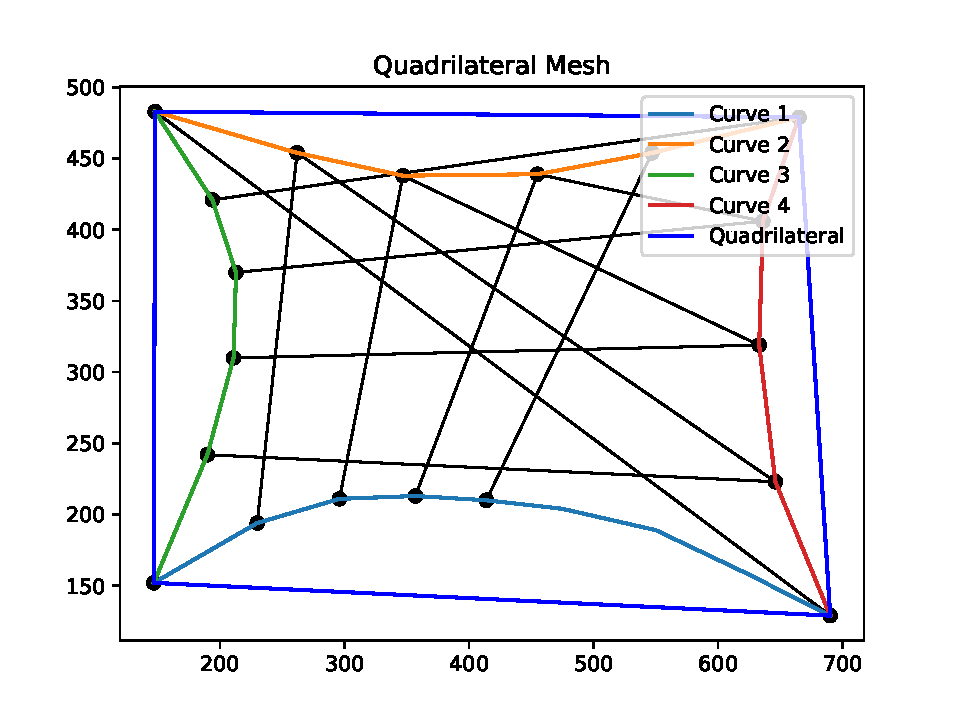
\includegraphics[scale=0.6]{quadrilateral_mesh_1.pdf}
\end{figure}

\begin{figure}[H]
  \centering
  \caption{Mapeamento paramétrico e projetor bilinear para as Curvas 2}
  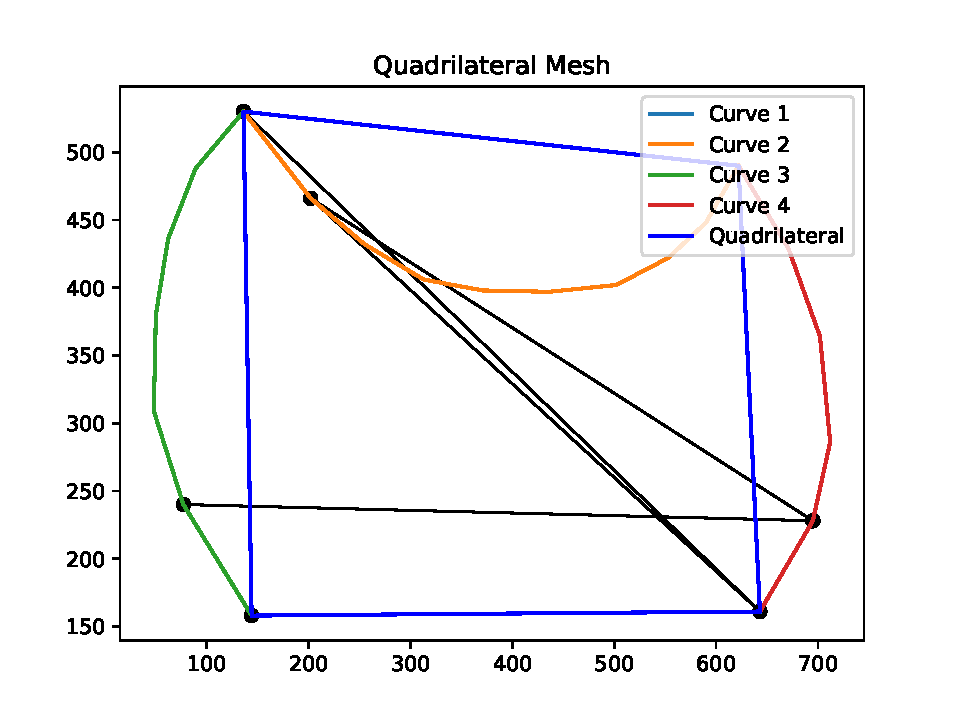
\includegraphics[scale=0.6]{quadrilateral_mesh_2.pdf}
\end{figure}

\section{Conclusão}

Este trabalho apresentou uma aplicação de um projetor bilinear para a geração de malha em um quadrilátero. 


\end{document}